\documentclass[11pt]{article}

\usepackage{latexsym}
\usepackage{graphicx}
\usepackage{amssymb}
\usepackage{amsthm}
\usepackage{enumerate}
\usepackage{amsmath}
\usepackage{cancel}
\numberwithin{equation}{section}
\numberwithin{figure}{section}
\numberwithin{table}{section}

\setlength{\evensidemargin}{.25in}
\setlength{\oddsidemargin}{-.25in}
\setlength{\topmargin}{-.75in}
\setlength{\textwidth}{6.5in}
\setlength{\textheight}{9.5in}
\newcommand{\due}{March 4th, 2010}
\newcommand{\HWnum}{5}
\newcommand{\grad}{\bold\nabla}
\newcommand{\vecE}{\vec{E}}
\newcommand{\scrptR}{\vec{\mathfrak{R}}}
\newcommand{\kapa}{\frac{1}{4\pi\epsilon_0}}
\newcommand{\unit}[1]{\ensuremath{\, \mathrm{#1}}}

\begin{document}
\begin{titlepage}
\setlength{\topmargin}{1.5in}
\begin{center}
\Huge{Physics 3320} \\
\LARGE{Principles of Electricity and Magnetism II} \\
\Large{Professor Ana Maria Rey} \\[1cm]

\huge{Homework \#\HWnum}\\[0.5cm]

\large{Joe Becker} \\
\large{SID: 810-07-1484} \\
\large{\due} 

\end{center}

\end{titlepage}



\section{Introduction}
Often we need to detect differing intensities of light in physical experiments and in communications. To do this we need to construct a photometer or an optical detector. To do this we will need to use a photodiode. This lab will explore differing properties of photodiodes and photometers.

\section{Theory}
The photometer used in this experiment is a current to voltage amplifier circuit. We used an op-amp to meet this end see figure \ref{FigPhotoDetec}.
\begin{figure}[h]
\centering
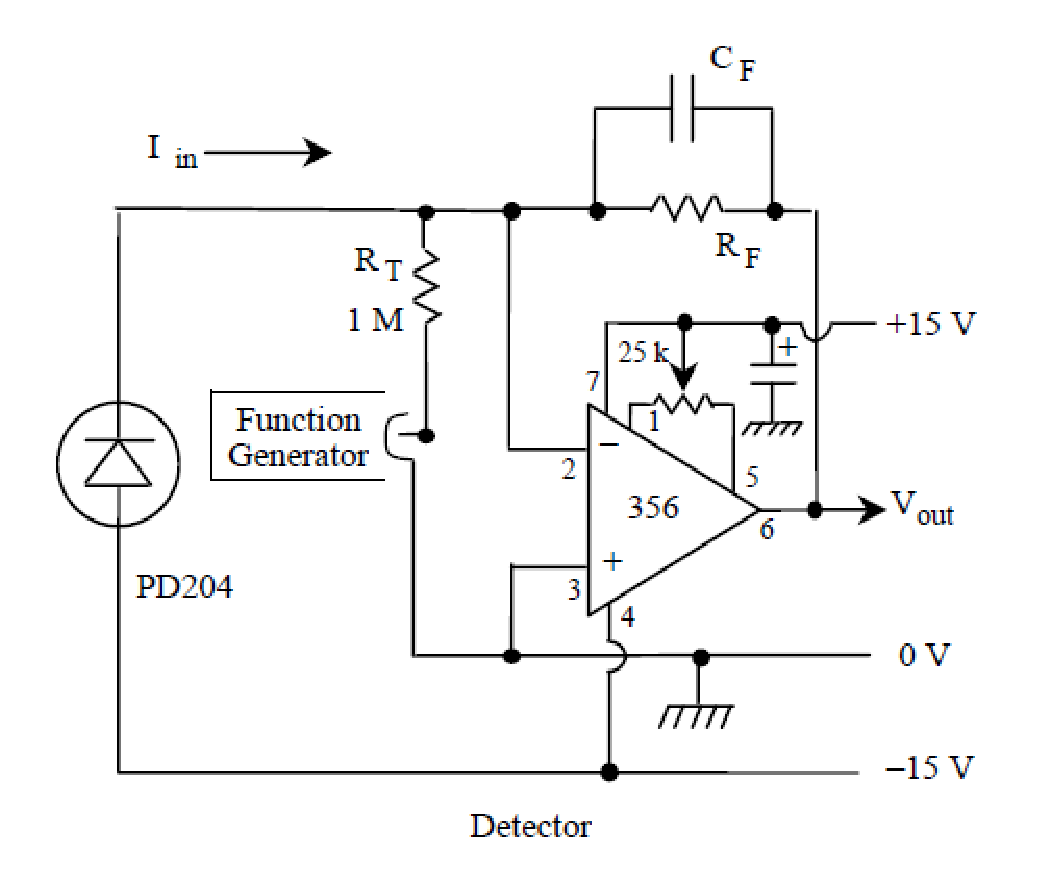
\includegraphics[scale=0.75]{FigPhotoDetec.eps}
\caption{\textit{The schematic for the photometer.}}
\label{FigPhotoDetec}
\end{figure}
Assuming the golden rules for an op-amp we can see that the output voltage is given by
\begin{equation}
V_{out} = -I_{in}R_F
\label{OutVolt}
\end{equation}
So we can say that the gain is 
\begin{equation}
G = \frac{V_{out}}{I_{in}} = -R_F
\label{Gain}
\end{equation}
We see from figure \ref{FigPhotoDetec} that the photodiode determines the input current, $I_{in}$. So we can say that the current generated by the photodiode is
\begin{equation}
I_{in} = S_{\lambda}N
\label{PhotoCurr}
\end{equation}
Where $N$ is the light intensity and $S_{\lambda}$ is the photodiode sensitivity and has a given value for a given wavelength $\lambda$ as
\begin{equation}
S_{\lambda} = R_{940\unit{nm}}RSR(\lambda)
\label{Sens}
\end{equation}
Where $R_{940\unit{nm}}$ is the peak sensitivity at $\lambda = 940\unit{nm}$ and has a given value as
$$R_{940\unit{nm}} = \frac{15\unit{\mu A}}{5\unit{mW/cm^2}} = 3\unit{\mu A/(mW/cm^2)}$$
for the PD204 photodiode. And $RSR(\lambda)$ is the relative spectral sensitivity which varies depending on the wavelength of light we are looking at. So if we solve equations \ref{PhotoCurr} and \ref{Sens} in terms of $N$ we get
\begin{equation}
N = \frac{V_{out}}{I_{in}S_{\lambda}}
\label{LightInten}
\end{equation}
So we now have a relation between the output voltage and the light intensity, now we can measure the intensity of light. 

For the MV5752 LED the intensity of the light it produces is given by
\begin{equation}
N = \frac{J(\unit{mW/str})}{r^2}
\label{LED}
\end{equation}
where $J$ is given as $J(\unit{mW/str}) = 1.1\unit{mW/str}$ and $r$ is the distance from the LED to the point of interest.

\section{Experiment}
To begin we built the circuit in figure \ref{FigPhotoDetec} where $C_F = 9.92\unit{pF}$, $R_T = 1.00\unit{M\Omega}$, and $R_F = 1.00\unit{M\Omega}$. We used $\pm15\unit{V}$ from the DC power supply to power the op-amp, and we used the function generator to create our input signals. The output from both the circuit and from the function generator were sent to the oscilloscope.

Then to test that the gain was negative one we covered the photodiode and sent a square wave with a frequency of $1.0\unit{kHz}$. We saw that the output voltage was inverted from the input with the same amplitude. So we got the expected gain of $-1$. 

Next we removed the voltage input from the circuit and uncovered the photodiode. Now the only current that is driving the circuit is the current from the phorodiode. Now we just let the photodiode absorb the fluorescent light in the lab. We measured the output voltage using the oscilloscopes cursors. We found that for the fluorescent light the output voltage was $V_{out} = 630\unit{mV}$. So if we assume that the wavelength of the light in the lab is $\lambda = 550\unit{nm}$ we can say that $RSR(550) = 0.70$ and we calculate $S_{\lambda=550\unit{nm}} = 2.1\unit{\mu A/(mW/cm^2)}$. Using the measured values for $V_{out}$ and $R_F$ we can use equation \ref{LightInten} to calculate $N = 0.30\unit{mW/cm^2}$. Now given that daylight has an intensity of $N_{daylight} = 100\unit{mW/cm^2}$ we see that the light in the lab is much less intense than the natural light from the sun. 

Next we measured the intensity of light reflected off of a sheet of white paper using both a calibrated light meter and the photometer we built. The output voltage we measured from the white piece of paper was $V_{out} = 330\unit{mV}$ using $S_{\lambda=550\unit{nm}}=2.1\unit{\mu A/(mW/cm^2)}$ and equation \ref{LightInten} we found that $N = 0.157\unit{mW/cm^2}$. Now we placed the light meter at the same distance from the paper as the photodiode and found that the intensity was $N = 13\unit{\mu W/cm^2} = 0.13\unit{mW/cm^2}$. So our circuit is near the sensitivity of the light meter.

For the next part of the experiment we first built the circuit in figure \ref{FigPhotoEmit} where $R_s = 178\unit{\Omega}$.
\begin{figure}[h]
\centering
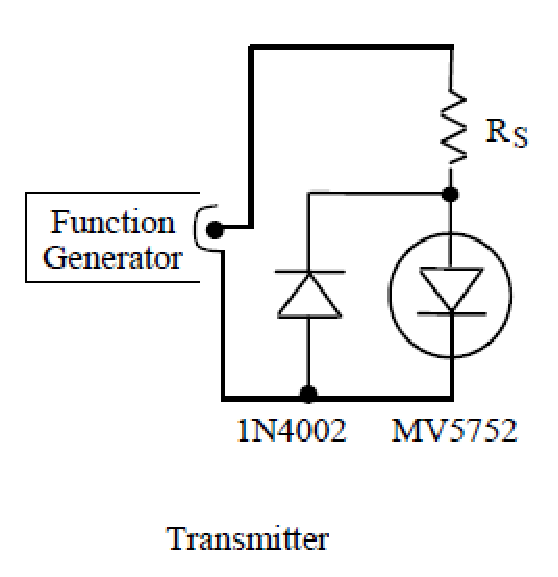
\includegraphics[scale=0.75]{FigPhotoEmit.eps}
\caption{\textit{The schematic for the light emitter.}}
\label{FigPhotoEmit}
\end{figure}
We then sent a square wave into the LED circuit with a amplitude of $4.0\unit{V_{pp}}$ with a voltage offset of $+2.0\unit{V}$ so the pulse varied from $0\unit{V}$ to $4\unit{V}$. Next we placed the LED $7.5\unit{cm}$ away from the photodiode and measured the output from out detector circuit as $V_{out} = 344\unit{mV}$ Now we assume that the wavelength of the light emitted from the LED is $\lambda = 635\unit{nm}$ so we calculated $S_{\lambda}$ from equation \ref{Sens} as $S_{\lambda=635\unit{nm}} = 2.4\unit{\mu A/(mW/cm^2)}$. So using $V_{out} = 344\unit{mV}$ and equation \ref{LightInten} we found that $N = 0.143\unit{mW/cm^2}$. Now using equation \ref{LED} and the fact that $r=7.5\unit{cm}$ we found that $N=0.13$ we see that these values agree.

We then found the exponential rise time of the output square wave. To do this we found the time it took for the waveform to rise to $67\%$ of the maximum output voltage. Using the oscilloscopes cursors we found $t_R = 62.0\unit{\mu s}$.

Next we split the output signal from the circuit to the oscilloscope and to a lock-in amplifier. We found that the lock-in amplifier is much more sensitive than the oscilloscope. We lost signal on the oscilloscope when the LED was $35\unit{cm}$ away from the photodiode. On the other the lock-in amplifier still read a signal of $63.9\unit{V}$. Note that we could not pull the LED far enough away to drop the signal off as our wire leads are not long enough to get the signal to drop off. The distance from the LED to the photodiode was $1.00\unit{m}$.

\section{Conclusion}
In conclusion we found that a photodiode can measure the intensity of light effectively. Much like a fiber optic cable we sent a signal using pulses of light, and on the other end we found that the signal the photodiode received the signal with very little delay (the exponential rise time was very small).
\end{document}

